\documentclass[16pt]{beamer}
\usepackage[utf8]{inputenc}
\usepackage[T1]{fontenc}
\usepackage{graphicx}
\usepackage[polish]{babel}
\usepackage{polski}
\usepackage{color}

\usetheme{Pittsburgh}
\usenavigationsymbolstemplate{} % turn off navigation icons
\setbeamercovered{transparent}

\usepackage{fancyvrb}
\usepackage{color}

\newcommand\at{@}
\newcommand\lb{[}
\newcommand\rb{]}
\newcommand\PYbg[1]{\textcolor[rgb]{0.00,0.50,0.00}{\textbf{#1}}}
\newcommand\PYbf[1]{\textcolor[rgb]{0.73,0.40,0.53}{\textbf{#1}}}
\newcommand\PYbe[1]{\textcolor[rgb]{0.40,0.40,0.40}{#1}}
\newcommand\PYbd[1]{\textcolor[rgb]{0.73,0.13,0.13}{#1}}
\newcommand\PYbc[1]{\textcolor[rgb]{0.00,0.50,0.00}{\textbf{#1}}}
\newcommand\PYbb[1]{\textcolor[rgb]{0.40,0.40,0.40}{#1}}
\newcommand\PYba[1]{\textcolor[rgb]{0.00,0.00,0.50}{\textbf{#1}}}
\newcommand\PYaJ[1]{\textcolor[rgb]{0.73,0.13,0.13}{#1}}
\newcommand\PYaK[1]{\textcolor[rgb]{0.00,0.00,1.00}{#1}}
\newcommand\PYaH[1]{\fcolorbox[rgb]{1.00,0.00,0.00}{1,1,1}{#1}}
\newcommand\PYaI[1]{\textcolor[rgb]{0.69,0.00,0.25}{#1}}
\newcommand\PYaN[1]{\textcolor[rgb]{0.00,0.00,1.00}{\textbf{#1}}}
\newcommand\PYaO[1]{\textcolor[rgb]{0.00,0.00,0.50}{\textbf{#1}}}
\newcommand\PYaL[1]{\textcolor[rgb]{0.73,0.73,0.73}{#1}}
\newcommand\PYaM[1]{\textcolor[rgb]{0.74,0.48,0.00}{#1}}
\newcommand\PYaB[1]{\textcolor[rgb]{0.00,0.25,0.82}{#1}}
\newcommand\PYaC[1]{\textcolor[rgb]{0.67,0.13,1.00}{#1}}
\newcommand\PYaA[1]{\textcolor[rgb]{0.00,0.50,0.00}{#1}}
\newcommand\PYaF[1]{\textcolor[rgb]{1.00,0.00,0.00}{#1}}
\newcommand\PYaG[1]{\textcolor[rgb]{0.10,0.09,0.49}{#1}}
\newcommand\PYaD[1]{\textcolor[rgb]{0.25,0.50,0.50}{\textit{#1}}}
\newcommand\PYaE[1]{\textcolor[rgb]{0.63,0.00,0.00}{#1}}
\newcommand\PYaZ[1]{\textcolor[rgb]{0.00,0.50,0.00}{\textbf{#1}}}
\newcommand\PYaX[1]{\textcolor[rgb]{0.00,0.50,0.00}{#1}}
\newcommand\PYaY[1]{\textcolor[rgb]{0.73,0.13,0.13}{#1}}
\newcommand\PYaR[1]{\textcolor[rgb]{0.10,0.09,0.49}{#1}}
\newcommand\PYaS[1]{\textcolor[rgb]{0.25,0.50,0.50}{\textit{#1}}}
\newcommand\PYaP[1]{\textcolor[rgb]{0.49,0.56,0.16}{#1}}
\newcommand\PYaQ[1]{\textcolor[rgb]{0.40,0.40,0.40}{#1}}
\newcommand\PYaV[1]{\textcolor[rgb]{0.00,0.00,1.00}{\textbf{#1}}}
\newcommand\PYaW[1]{\textcolor[rgb]{0.73,0.13,0.13}{#1}}
\newcommand\PYaT[1]{\textcolor[rgb]{0.50,0.00,0.50}{\textbf{#1}}}
\newcommand\PYaU[1]{\textcolor[rgb]{0.82,0.25,0.23}{\textbf{#1}}}
\newcommand\PYaj[1]{\textcolor[rgb]{0.00,0.50,0.00}{#1}}
\newcommand\PYak[1]{\textcolor[rgb]{0.73,0.40,0.53}{#1}}
\newcommand\PYah[1]{\textcolor[rgb]{0.63,0.63,0.00}{#1}}
\newcommand\PYai[1]{\textcolor[rgb]{0.10,0.09,0.49}{#1}}
\newcommand\PYan[1]{\textcolor[rgb]{0.67,0.13,1.00}{\textbf{#1}}}
\newcommand\PYao[1]{\textcolor[rgb]{0.73,0.40,0.13}{\textbf{#1}}}
\newcommand\PYal[1]{\textcolor[rgb]{0.25,0.50,0.50}{\textit{#1}}}
\newcommand\PYam[1]{\textbf{#1}}
\newcommand\PYab[1]{\textit{#1}}
\newcommand\PYac[1]{\textcolor[rgb]{0.73,0.13,0.13}{#1}}
\newcommand\PYaa[1]{\textcolor[rgb]{0.50,0.50,0.50}{#1}}
\newcommand\PYaf[1]{\textcolor[rgb]{0.25,0.50,0.50}{\textit{#1}}}
\newcommand\PYag[1]{\textcolor[rgb]{0.40,0.40,0.40}{#1}}
\newcommand\PYad[1]{\textcolor[rgb]{0.73,0.13,0.13}{#1}}
\newcommand\PYae[1]{\textcolor[rgb]{0.40,0.40,0.40}{#1}}
\newcommand\PYaz[1]{\textcolor[rgb]{0.00,0.63,0.00}{#1}}
\newcommand\PYax[1]{\textcolor[rgb]{0.60,0.60,0.60}{\textbf{#1}}}
\newcommand\PYay[1]{\textcolor[rgb]{0.00,0.50,0.00}{\textbf{#1}}}
\newcommand\PYar[1]{\textcolor[rgb]{0.10,0.09,0.49}{#1}}
\newcommand\PYas[1]{\textcolor[rgb]{0.73,0.13,0.13}{\textit{#1}}}
\newcommand\PYap[1]{\textcolor[rgb]{0.00,0.50,0.00}{#1}}
\newcommand\PYaq[1]{\textcolor[rgb]{0.53,0.00,0.00}{#1}}
\newcommand\PYav[1]{\textcolor[rgb]{0.00,0.50,0.00}{\textbf{#1}}}
\newcommand\PYaw[1]{\textcolor[rgb]{0.40,0.40,0.40}{#1}}
\newcommand\PYat[1]{\textcolor[rgb]{0.10,0.09,0.49}{#1}}
\newcommand\PYau[1]{\textcolor[rgb]{0.40,0.40,0.40}{#1}}


\author{Śląska Grupa Użytkowników języka Ruby\\
  \footnotesize{Jakub Kuźma}}
\title{Podstawy tworzenia aplikacji internetowych z wykorzystaniem YUI 3 i Rails 3}

\begin{document}

\frame{\titlepage}

\begin{frame}
  \frametitle{Wstęp}
  \begin{center}
    Zaawansowana aplikacja internetowa?
  \end{center}
\end{frame}

\begin{frame}
  \frametitle{Brydż - licytacja}
  \begin{figure}
    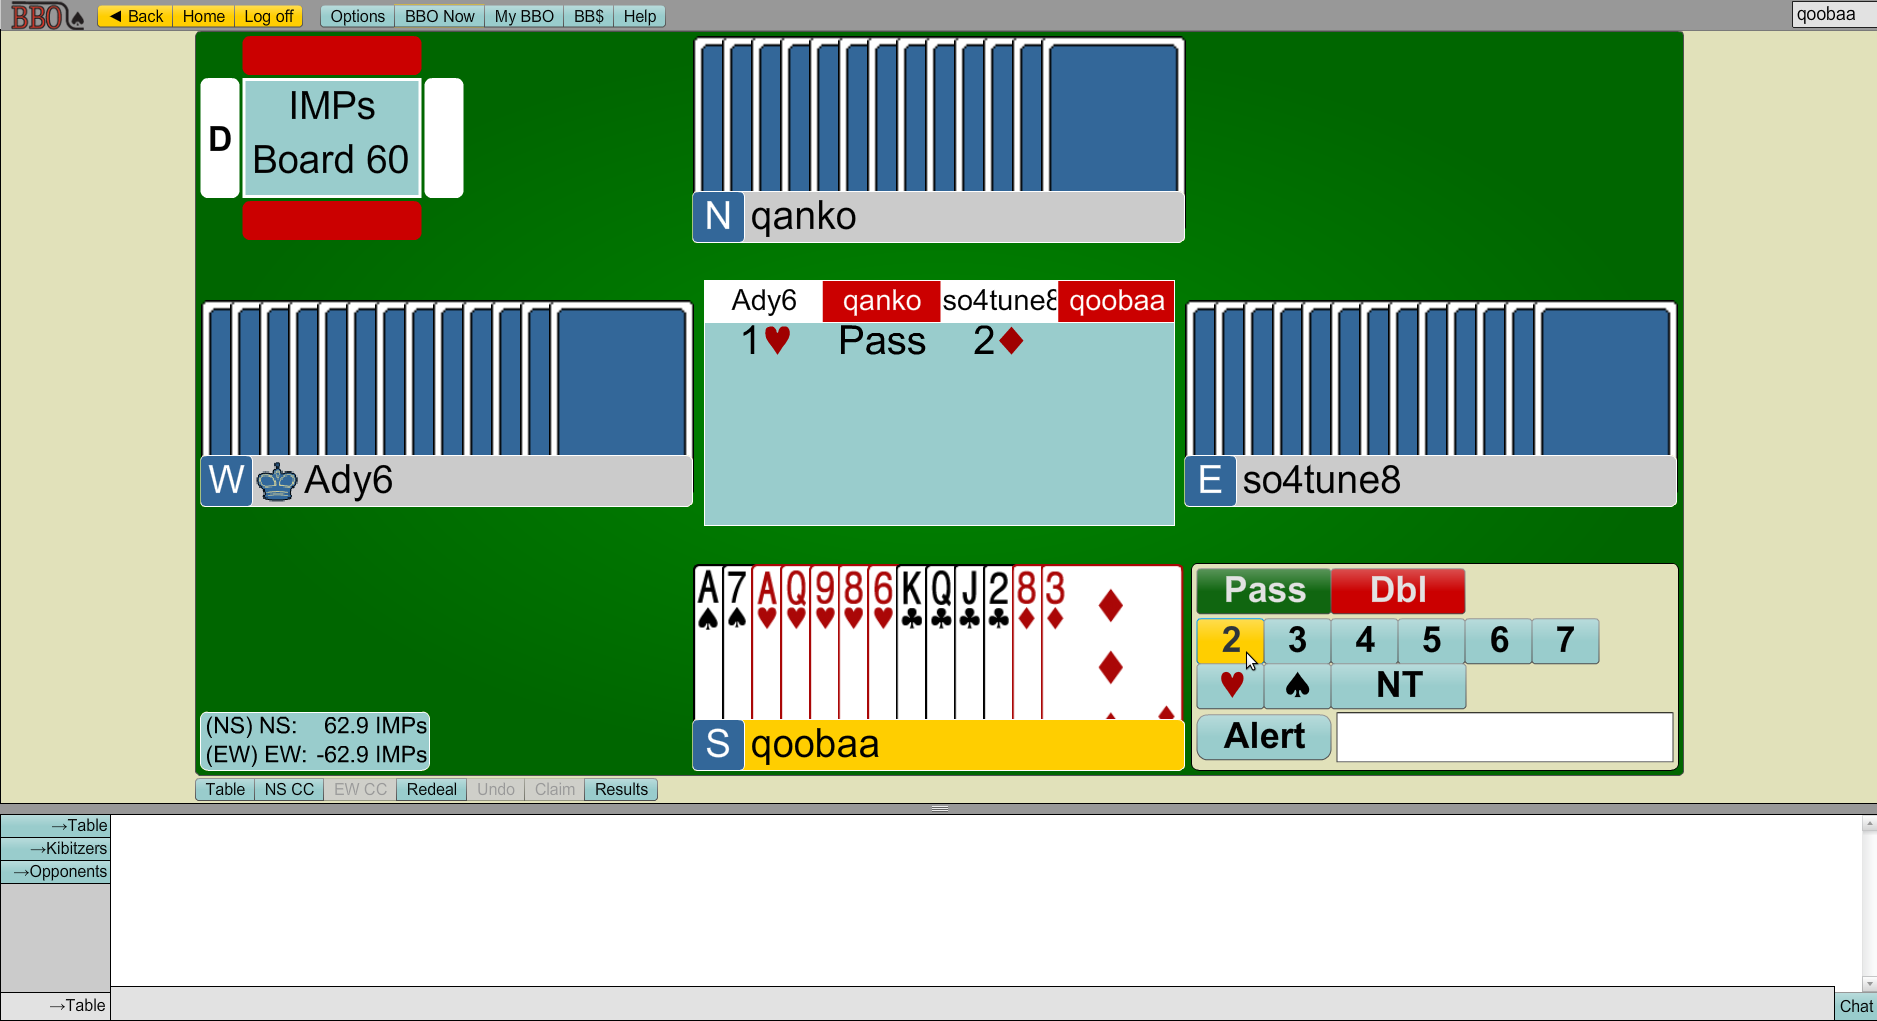
\includegraphics[width=\linewidth]{bbo-auction.png}
  \end{figure}
\end{frame}

\begin{frame}
  \frametitle{Brydż - rozgrywka}
  \begin{figure}
    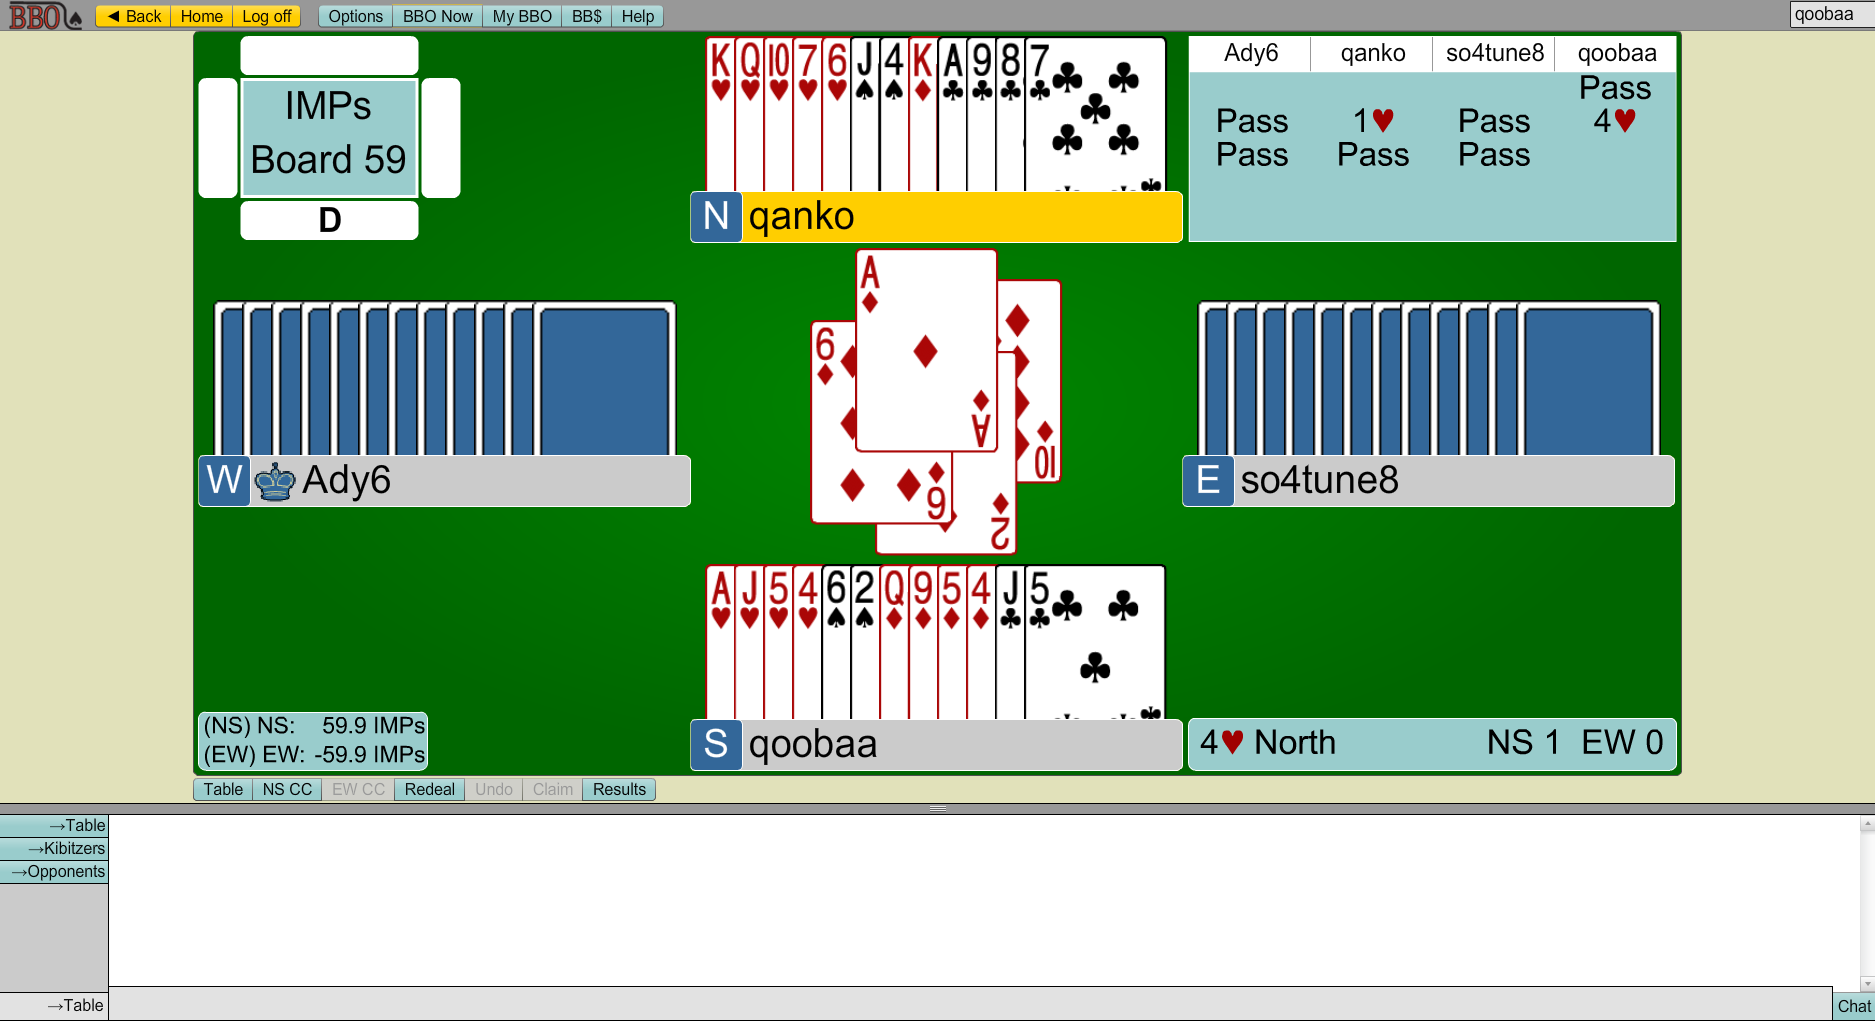
\includegraphics[width=\linewidth]{bbo-play.png}
  \end{figure}
\end{frame}

\begin{frame}
  \frametitle{Wymagania}
  \begin{itemize}
  \item komunikacja z serwerem bez przeładowania strony
  \item walidacja działań użytkownika przed wysłaniem żądania
  \item rozbicie interfejsu na małe, niezależne elementy
  \end{itemize}
\end{frame}

\begin{frame}
  \frametitle{jQuery}
  \begin{center}
    absurdalnie prosty AJAX, obsługa zdarzeń, manipulacja DOM
  \end{center}
\end{frame}

\begin{frame}
  \frametitle{jQuery UI}
  \begin{center}
    jQuery UI jest tym dla RIA, czym jQuery było dla AJAX
  \end{center}
\end{frame}

\begin{frame}
  \frametitle{YUI}
  \begin{figure}
    
\includegraphics[width=0.8\linewidth]{yui.jpg}
  \end{figure}
\end{frame}

\begin{frame}
  \frametitle{YUI 3 - w rolach głównych}
  \begin{itemize}
  \item Developer Tools
  \item Core
  \item Utilities
  \item Component Infrastructure
  \item Widgets
  \item Plugins
  \end{itemize}
\end{frame}

\begin{frame}
  \frametitle{Component Infrastructure}
  \begin{itemize}
  \item Attribute
  \item Base
  \item Widget
  \item Plugin
  \end{itemize}
\end{frame}

\begin{frame}
  \frametitle{Attribute}
  \begin{itemize}
  \item settery, gettery, walidatory
  \item zdarzenie attributeChanged
  \item klonowanie obiektów
  \item obsługa zagnieżdżonych wartości (np. strings.messages.hello)
  \end{itemize}
\end{frame}

\begin{frame}
  \frametitle{Base}
  \begin{itemize}
  \item konstruktor i destruktor
  \item atrybuty
  \item obsługa zdarzeń
  \item obsługa rozszerzeń i wtyczek
  \end{itemize}
\end{frame}

\begin{frame}
  \frametitle{Widget}
  \begin{itemize}
  \item HTML Parser
  \item renderUI
  \item bindUI
  \item syncUI
  \item boundingBox, contentBox
  \end{itemize}
\end{frame}

\begin{frame}
  \frametitle{Plugin}
  \begin{itemize}
  \item nieinwazyjne ,,wzbogacanie'' obiektów
  \item afterHostEvent, beforeHostMethod, itp.
  \end{itemize}
\end{frame}

\begin{frame}
  \frametitle{Custom Events}
  \begin{itemize}
  \item niezależne od DOM
  \item to samo API (bubbling - stopPropagation, defaultFn - preventDefault)
  \end{itemize}
\end{frame}

\begin{frame}
  \frametitle{Inne}
  \begin{itemize}
  \item operacje na tablicach (every, find, reduce, itp.)
  \item OOP (augment, extend, bind, rbind)
  \item YUI 3 Gallery
  \end{itemize}
\end{frame}

\begin{frame}
  \frametitle{Rails 3}
  \begin{itemize}
  \item logika gry - walidacja
  \item tradycyjny serwis webowy oraz API % respondery - zmiana pollingu na websockety
  \end{itemize}
\end{frame}

\begin{frame}
  \frametitle{node.js}
  \begin{itemize}
  \item YUI3 to CommonJS
  \item podmiana modułu Get
  \item obsługa DOM dzięki jsdom
  \end{itemize}
\end{frame}

\begin{frame}
  \frametitle{Warto zwrócić uwagę}
  \begin{itemize}
  \item underscore.js
  \item mustache.js
  \end{itemize}
\end{frame}

% slajd z Drogusem? :-)

\end{document}
